\begin{figure}[!htpb]
\centering
\resizebox{!}{7cm}{%


\tikzset{every picture/.style={line width=0.75pt}} %set default line width to 0.75pt        

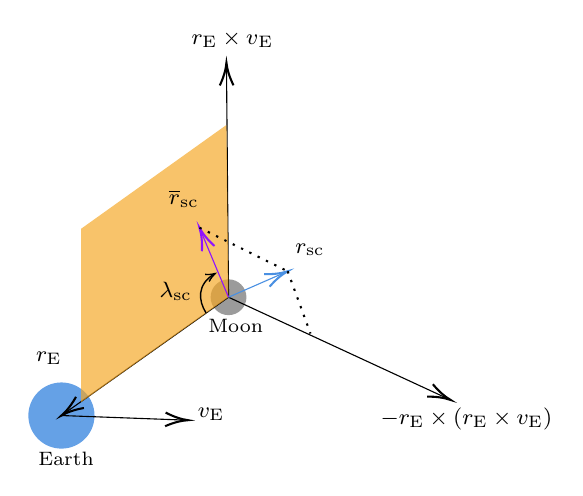
\begin{tikzpicture}[x=0.75pt,y=0.75pt,yscale=-1,xscale=1]
%uncomment if require: \path (0,275); %set diagram left start at 0, and has height of 275

%Shape: Circle [id:dp2824516770212466] 
\draw  [draw opacity=0][fill={rgb, 255:red, 74; green, 144; blue, 226 }  ,fill opacity=0.85 ] (4.56,190) .. controls (4.56,181.2) and (11.7,174.06) .. (20.5,174.06) .. controls (29.3,174.06) and (36.44,181.2) .. (36.44,190) .. controls (36.44,198.8) and (29.3,205.94) .. (20.5,205.94) .. controls (11.7,205.94) and (4.56,198.8) .. (4.56,190) -- cycle ;
%Shape: Circle [id:dp7791082362171957] 
\draw  [draw opacity=0][fill={rgb, 255:red, 155; green, 155; blue, 155 }  ,fill opacity=1 ] (92.38,133) .. controls (92.38,128.24) and (96.24,124.38) .. (101,124.38) .. controls (105.76,124.38) and (109.63,128.24) .. (109.63,133) .. controls (109.63,137.76) and (105.76,141.63) .. (101,141.63) .. controls (96.24,141.63) and (92.38,137.76) .. (92.38,133) -- cycle ;
%Straight Lines [id:da2577675215112112] 
\draw    (101,133) -- (100.02,22) ;
\draw [shift={(100,20)}, rotate = 89.49] [color={rgb, 255:red, 0; green, 0; blue, 0 }  ][line width=0.75]    (10.93,-3.29) .. controls (6.95,-1.4) and (3.31,-0.3) .. (0,0) .. controls (3.31,0.3) and (6.95,1.4) .. (10.93,3.29)   ;
%Straight Lines [id:da9217068766699217] 
\draw    (101,133) -- (206.18,181.66) ;
\draw [shift={(208,182.5)}, rotate = 204.83] [color={rgb, 255:red, 0; green, 0; blue, 0 }  ][line width=0.75]    (10.93,-3.29) .. controls (6.95,-1.4) and (3.31,-0.3) .. (0,0) .. controls (3.31,0.3) and (6.95,1.4) .. (10.93,3.29)   ;
%Straight Lines [id:da7702933848353208] 
\draw    (101,133) -- (22.13,188.84) ;
\draw [shift={(20.5,190)}, rotate = 324.7] [color={rgb, 255:red, 0; green, 0; blue, 0 }  ][line width=0.75]    (10.93,-3.29) .. controls (6.95,-1.4) and (3.31,-0.3) .. (0,0) .. controls (3.31,0.3) and (6.95,1.4) .. (10.93,3.29)   ;
%Shape: Polygon [id:ds9714041146034247] 
\draw  [draw opacity=0][fill={rgb, 255:red, 245; green, 166; blue, 35 }  ,fill opacity=0.68 ] (100,50) -- (101,133) -- (30,183.5) -- (30,100) -- cycle ;
%Straight Lines [id:da1524507160013362] 
\draw [color={rgb, 255:red, 74; green, 144; blue, 226 }  ,draw opacity=1 ]   (101,133) -- (127.67,121.3) ;
\draw [shift={(129.5,120.5)}, rotate = 156.32] [color={rgb, 255:red, 74; green, 144; blue, 226 }  ,draw opacity=1 ][line width=0.75]    (10.93,-3.29) .. controls (6.95,-1.4) and (3.31,-0.3) .. (0,0) .. controls (3.31,0.3) and (6.95,1.4) .. (10.93,3.29)   ;
%Straight Lines [id:da0032699970922163146] 
\draw [line width=0.75]  [dash pattern={on 0.84pt off 2.51pt}]  (129.5,120.5) -- (140.5,150.5) ;
%Straight Lines [id:da11822863801442884] 
\draw [color={rgb, 255:red, 144; green, 19; blue, 254 }  ,draw opacity=1 ]   (101,133) -- (87.77,101.35) ;
\draw [shift={(87,99.5)}, rotate = 67.32] [color={rgb, 255:red, 144; green, 19; blue, 254 }  ,draw opacity=1 ][line width=0.75]    (10.93,-3.29) .. controls (6.95,-1.4) and (3.31,-0.3) .. (0,0) .. controls (3.31,0.3) and (6.95,1.4) .. (10.93,3.29)   ;
%Straight Lines [id:da651317698755093] 
\draw [line width=0.75]  [dash pattern={on 0.84pt off 2.51pt}]  (87,99.5) -- (129.5,120.5) ;
%Straight Lines [id:da8371067193323121] 
\draw    (20.5,190) -- (79.5,192.18) ;
\draw [shift={(81.5,192.25)}, rotate = 182.11] [color={rgb, 255:red, 0; green, 0; blue, 0 }  ][line width=0.75]    (10.93,-3.29) .. controls (6.95,-1.4) and (3.31,-0.3) .. (0,0) .. controls (3.31,0.3) and (6.95,1.4) .. (10.93,3.29)   ;
%Curve Lines [id:da7207911345943288] 
\draw   [line width=0.5] (90.21,140.63) .. controls (86.43,134.66) and (85.56,126.72) .. (94.56,121.57) ;
\draw [shift={(94.53,121.61)}, rotate = 151.07] [color={rgb, 255:red, 0; green, 0; blue, 0 }  ][line width=0.5]    (4.37,-1.96) .. controls (2.78,-0.92) and (1.32,-0.27) .. (0,0) .. controls (1.32,0.27) and (2.78,0.92) .. (4.37,1.96)   ;

% Text Node
\draw (71,79.9) node [anchor=north west][inner sep=0.75pt]  [font=\footnotesize]  {$\overline{r}_{\mathrm{sc}}$};
% Text Node
\draw (132,105.9) node [anchor=north west][inner sep=0.75pt]  [font=\footnotesize]  {$r_{\mathrm{sc}}$};
% Text Node
\draw (7,157.9) node [anchor=north west][inner sep=0.75pt]  [font=\footnotesize]  {$r_{\mathrm{{ E}}}$};
% Text Node
\draw (82,3.4) node [anchor=north west][inner sep=0.75pt]  [font=\footnotesize]  {$r_{\mathrm{{ E}}} \times v\mathrm{_{E}}$};
% Text Node
\draw (4.5,206.5) node [anchor=north west][inner sep=0.75pt]  [font=\scriptsize] [align=left] {\text{ Earth}};
% Text Node
\draw (85,184.9) node [anchor=north west][inner sep=0.75pt]  [font=\footnotesize]  {$v_{\mathrm{{ E}}}$};
% Text Node
\draw (173,184.9) node [anchor=north west][inner sep=0.75pt]  [font=\footnotesize]  {$-r_{\mathrm{{ E}}} \times ( r_{\mathrm{{ E}}} \times v_{\mathrm{{ E}}})$};
% Text Node
\draw (90,142.5) node [anchor=north west][inner sep=0.75pt]  [font=\footnotesize] [align=left] {{\scriptsize \text{Moon}}};
% Text Node
\draw (66.5,124.4) node [anchor=north west][inner sep=0.75pt]  [font=\footnotesize]  {$\lambda _{\mathrm{sc}}$};


\end{tikzpicture}%
}
\end{figure}

